\documentclass[11pt,]{article}
\usepackage[left=1in,top=1in,right=1in,bottom=1in]{geometry}
\newcommand*{\authorfont}{\fontfamily{phv}\selectfont}
\usepackage[]{mathpazo}


  \usepackage[T1]{fontenc}
  \usepackage[utf8]{inputenc}




\usepackage{abstract}
\renewcommand{\abstractname}{}    % clear the title
\renewcommand{\absnamepos}{empty} % originally center

\renewenvironment{abstract}
 {{%
    \setlength{\leftmargin}{0mm}
    \setlength{\rightmargin}{\leftmargin}%
  }%
  \relax}
 {\endlist}

\makeatletter
\def\@maketitle{%
  \newpage
%  \null
%  \vskip 2em%
%  \begin{center}%
  \let \footnote \thanks
    {\fontsize{18}{20}\selectfont\raggedright  \setlength{\parindent}{0pt} \@title \par}%
}
%\fi
\makeatother




\setcounter{secnumdepth}{0}

\usepackage{color}
\usepackage{fancyvrb}
\newcommand{\VerbBar}{|}
\newcommand{\VERB}{\Verb[commandchars=\\\{\}]}
\DefineVerbatimEnvironment{Highlighting}{Verbatim}{commandchars=\\\{\}}
% Add ',fontsize=\small' for more characters per line
\usepackage{framed}
\definecolor{shadecolor}{RGB}{248,248,248}
\newenvironment{Shaded}{\begin{snugshade}}{\end{snugshade}}
\newcommand{\AlertTok}[1]{\textcolor[rgb]{0.94,0.16,0.16}{#1}}
\newcommand{\AnnotationTok}[1]{\textcolor[rgb]{0.56,0.35,0.01}{\textbf{\textit{#1}}}}
\newcommand{\AttributeTok}[1]{\textcolor[rgb]{0.77,0.63,0.00}{#1}}
\newcommand{\BaseNTok}[1]{\textcolor[rgb]{0.00,0.00,0.81}{#1}}
\newcommand{\BuiltInTok}[1]{#1}
\newcommand{\CharTok}[1]{\textcolor[rgb]{0.31,0.60,0.02}{#1}}
\newcommand{\CommentTok}[1]{\textcolor[rgb]{0.56,0.35,0.01}{\textit{#1}}}
\newcommand{\CommentVarTok}[1]{\textcolor[rgb]{0.56,0.35,0.01}{\textbf{\textit{#1}}}}
\newcommand{\ConstantTok}[1]{\textcolor[rgb]{0.00,0.00,0.00}{#1}}
\newcommand{\ControlFlowTok}[1]{\textcolor[rgb]{0.13,0.29,0.53}{\textbf{#1}}}
\newcommand{\DataTypeTok}[1]{\textcolor[rgb]{0.13,0.29,0.53}{#1}}
\newcommand{\DecValTok}[1]{\textcolor[rgb]{0.00,0.00,0.81}{#1}}
\newcommand{\DocumentationTok}[1]{\textcolor[rgb]{0.56,0.35,0.01}{\textbf{\textit{#1}}}}
\newcommand{\ErrorTok}[1]{\textcolor[rgb]{0.64,0.00,0.00}{\textbf{#1}}}
\newcommand{\ExtensionTok}[1]{#1}
\newcommand{\FloatTok}[1]{\textcolor[rgb]{0.00,0.00,0.81}{#1}}
\newcommand{\FunctionTok}[1]{\textcolor[rgb]{0.00,0.00,0.00}{#1}}
\newcommand{\ImportTok}[1]{#1}
\newcommand{\InformationTok}[1]{\textcolor[rgb]{0.56,0.35,0.01}{\textbf{\textit{#1}}}}
\newcommand{\KeywordTok}[1]{\textcolor[rgb]{0.13,0.29,0.53}{\textbf{#1}}}
\newcommand{\NormalTok}[1]{#1}
\newcommand{\OperatorTok}[1]{\textcolor[rgb]{0.81,0.36,0.00}{\textbf{#1}}}
\newcommand{\OtherTok}[1]{\textcolor[rgb]{0.56,0.35,0.01}{#1}}
\newcommand{\PreprocessorTok}[1]{\textcolor[rgb]{0.56,0.35,0.01}{\textit{#1}}}
\newcommand{\RegionMarkerTok}[1]{#1}
\newcommand{\SpecialCharTok}[1]{\textcolor[rgb]{0.00,0.00,0.00}{#1}}
\newcommand{\SpecialStringTok}[1]{\textcolor[rgb]{0.31,0.60,0.02}{#1}}
\newcommand{\StringTok}[1]{\textcolor[rgb]{0.31,0.60,0.02}{#1}}
\newcommand{\VariableTok}[1]{\textcolor[rgb]{0.00,0.00,0.00}{#1}}
\newcommand{\VerbatimStringTok}[1]{\textcolor[rgb]{0.31,0.60,0.02}{#1}}
\newcommand{\WarningTok}[1]{\textcolor[rgb]{0.56,0.35,0.01}{\textbf{\textit{#1}}}}

\usepackage{graphicx,grffile}
\makeatletter
\def\maxwidth{\ifdim\Gin@nat@width>\linewidth\linewidth\else\Gin@nat@width\fi}
\def\maxheight{\ifdim\Gin@nat@height>\textheight\textheight\else\Gin@nat@height\fi}
\makeatother
% Scale images if necessary, so that they will not overflow the page
% margins by default, and it is still possible to overwrite the defaults
% using explicit options in \includegraphics[width, height, ...]{}
\setkeys{Gin}{width=\maxwidth,height=\maxheight,keepaspectratio}


\title{Programación Estadística: Bisección  }



\author{\Large Adrián Sosa\vspace{0.05in} \newline\normalsize\emph{}   \and \Large \vspace{0.05in} \newline\normalsize\emph{Universidad Veracruzana}  }



\date{}

\usepackage{titlesec}

\titleformat*{\section}{\normalsize\bfseries}
\titleformat*{\subsection}{\normalsize\itshape}
\titleformat*{\subsubsection}{\normalsize\itshape}
\titleformat*{\paragraph}{\normalsize\itshape}
\titleformat*{\subparagraph}{\normalsize\itshape}


\usepackage{natbib}
\bibliographystyle{plainnat}
\usepackage[strings]{underscore} % protect underscores in most circumstances



\newtheorem{hypothesis}{Hypothesis}
\usepackage{setspace}


% set default figure placement to htbp
\makeatletter
\def\fps@figure{htbp}
\makeatother

\usepackage{hyperref}

% move the hyperref stuff down here, after header-includes, to allow for - \usepackage{hyperref}

\makeatletter
\@ifpackageloaded{hyperref}{}{%
\ifxetex
  \PassOptionsToPackage{hyphens}{url}\usepackage[setpagesize=false, % page size defined by xetex
              unicode=false, % unicode breaks when used with xetex
              xetex]{hyperref}
\else
  \PassOptionsToPackage{hyphens}{url}\usepackage[draft,unicode=true]{hyperref}
\fi
}

\@ifpackageloaded{color}{
    \PassOptionsToPackage{usenames,dvipsnames}{color}
}{%
    \usepackage[usenames,dvipsnames]{color}
}
\makeatother
\hypersetup{breaklinks=true,
            bookmarks=true,
            pdfauthor={Adrián Sosa () and  (Universidad Veracruzana)},
            pdfkeywords = {},  
            pdftitle={Programación Estadística: Bisección},
            colorlinks=true,
            citecolor=blue,
            urlcolor=blue,
            linkcolor=magenta,
            pdfborder={0 0 0}}
\urlstyle{same}  % don't use monospace font for urls

% Add an option for endnotes. -----


% add tightlist ----------
\providecommand{\tightlist}{%
\setlength{\itemsep}{0pt}\setlength{\parskip}{0pt}}

% add some other packages ----------

% \usepackage{multicol}
% This should regulate where figures float
% See: https://tex.stackexchange.com/questions/2275/keeping-tables-figures-close-to-where-they-are-mentioned
\usepackage[section]{placeins}


\begin{document}
	
% \pagenumbering{arabic}% resets `page` counter to 1 
%
% \maketitle

{% \usefont{T1}{pnc}{m}{n}
\setlength{\parindent}{0pt}
\thispagestyle{plain}
{\fontsize{18}{20}\selectfont\raggedright 
\maketitle  % title \par  

}

{
   \vskip 13.5pt\relax \normalsize\fontsize{11}{12} 
\textbf{\authorfont Adrián Sosa} \hskip 15pt \emph{\small }   \par \textbf{\authorfont } \hskip 15pt \emph{\small Universidad Veracruzana}   
}

}






\vskip -8.5pt


 % removetitleabstract

\noindent  

\hypertarget{bisecciuxf3n}{%
\subsection{Bisección}\label{bisecciuxf3n}}

El método de bisección es uno de los más versátiles para determinar una
raíz real en un intervalo de una ecuación dada, es fácil de comprender,
aunque si se desea una mayor exactitud el número de cálculos que hay que
realizar aumenta considerablemente.

El método de bisección se basa en el Teorema de Bolzano, el cual afirma
que si se tiene una función real \(y = f(x)\) continua en el intervalo
\(\textbf{[a,b]}\) donde el signo de la función en el extremo
\(\textbf{a}\) es distinto al signo de la función en el extremo
\(\textbf{b}\) del intervalo, entonces existe al menos un
\(c \in [a,b] | f(c)=0\) , que es la raíz buscada.

\hypertarget{procedimiento}{%
\subsubsection{Procedimiento}\label{procedimiento}}

\begin{itemize}
\tightlist
\item
  Debe existir seguridad sobre la continuidad de \(f(x)\) sobre el
  segmento \([a,b]\).
\item
  Se verifica que \(f(a)f(b)<0\).
\item
  Se calcula el punto medio m en el intervalo \([a,b]\) y se evalúa
  \(f(m)\) si ese valor es igual a 0 ya se ha encontrado la raíz.
\item
  En caso contrario se verifica si \(f(m)\) tiene signo opuesto con
  \(f(a)\) o con \(f(b)\).
\item
  se redefine el intervalo \([a,b]\) como\$ {[}a,m{]}\$ o \([m,b]\)
  según se haya determinado en cual de los casos haya el cambio de
  signo.
\item
  Con este nuevo intervalo se continúa sucesivamente encerrando la
  solución en un intervalo cada vez más pequeño, hasta alcanzar la
  precisión deseada
\end{itemize}

\hypertarget{ventajas}{%
\subsubsection{Ventajas}\label{ventajas}}

\begin{itemize}
\tightlist
\item
  Es siempre convergente.
\item
  Es óptimo para resolver una~ecuación~\(f(x)=0\)~cuando no se sabe nada
  de~\(f\), excepto calcular su signo.
\item
  Requiere que~\(f\)~sea continua en el~intervalo~especificado.
\item
  Se puede establecer el límite de error.
\item
  Es fácil de implementar.
\end{itemize}

\hypertarget{desventajas}{%
\subsubsection{Desventajas}\label{desventajas}}

\begin{itemize}
\tightlist
\item
  Converge muy lentamente.
\item
  Permite encontrar solo una~raíz, aunque existan más en el~intervalo.
\item
  Algunas veces la determinación del~intervalo~inicial no es muy fácil.
\item
  No puede determinar raíces complejas.
\item
  Es difícil generalizarlo para dimensiones superiores.
\end{itemize}

\newpage

\hypertarget{codificaciuxf3n}{%
\subsubsection{Codificación}\label{codificaciuxf3n}}

El método de bisección es relativamente sencillo de implementar:

\begin{verbatim}
## function (Fx, limI, limS, tol = 1e-06) 
## {
##     repeat {
##         x <- (limI + limS)/2
##         L <- (limS - limI)/2
##         if (Fx(x) == 0) {
##             return(x)
##             break
##         }
##         else if (Fx(limI) * Fx(x) < 0) {
##             limS <- x
##         }
##         else {
##             limI <- x
##         }
##         if (L < tol) {
##             return(x)
##             break
##         }
##     }
## }
\end{verbatim}

Para utilizarlo debemos definir una función para encontrar su ráiz y un
espacio de búsqueda:

\begin{Shaded}
\begin{Highlighting}[]
\NormalTok{fx1}
\end{Highlighting}
\end{Shaded}

\begin{verbatim}
## function (x) 
## {
##     return(x^2 + 3 * x - 2)
## }
\end{verbatim}

\begin{Shaded}
\begin{Highlighting}[]
\CommentTok{# se definen los límites}
\NormalTok{limS <-}\StringTok{ }\DecValTok{10}
\NormalTok{limI <-}\StringTok{ }\DecValTok{-10}
\NormalTok{steps <-}\StringTok{ }\FloatTok{0.01}
\CommentTok{# se crea el espacio de búsqueda}
\NormalTok{x <-}\StringTok{ }\KeywordTok{seq}\NormalTok{(limI, limS, steps)}
\NormalTok{y <-}\StringTok{ }\KeywordTok{c}\NormalTok{()}
\ControlFlowTok{for}\NormalTok{ (i }\ControlFlowTok{in} \KeywordTok{seq_along}\NormalTok{(x))\{y[i] <-}\StringTok{ }\KeywordTok{fx1}\NormalTok{(x[i])\}}
\CommentTok{# se optiene la ráiz}
\NormalTok{ráiz <-}\StringTok{ }\KeywordTok{biseccion}\NormalTok{(fx1, limI, limS)}
\end{Highlighting}
\end{Shaded}

El resultado se almacenara en la variable \emph{ráiz}, para conocerlo
basta con imprimirlo:

\begin{Shaded}
\begin{Highlighting}[]
\NormalTok{ráiz}
\end{Highlighting}
\end{Shaded}

\begin{verbatim}
## [1] -3.561553
\end{verbatim}

Si deseamos podémos gráficar la función y nuestro resultado.

\begin{Shaded}
\begin{Highlighting}[]
\CommentTok{# se crea un dataframe}
\NormalTok{df <-}\StringTok{ }\KeywordTok{data.frame}\NormalTok{(x,y)  }
\KeywordTok{ggplot}\NormalTok{(}\DataTypeTok{data=}\NormalTok{ df, }\DataTypeTok{mapping=}\KeywordTok{aes}\NormalTok{(}\DataTypeTok{x=}\NormalTok{ x, }\DataTypeTok{y =}\NormalTok{y))}\OperatorTok{+}
\StringTok{  }\KeywordTok{geom_line}\NormalTok{(}\DataTypeTok{color=}\DecValTok{4}\NormalTok{)}\OperatorTok{+}
\StringTok{  }\KeywordTok{annotate}\NormalTok{(}\DataTypeTok{geom=}\StringTok{"text"}\NormalTok{,}\DataTypeTok{x=}\NormalTok{ráiz}\DecValTok{-2}\NormalTok{, }\DataTypeTok{y=}\DecValTok{0}\NormalTok{, }\DataTypeTok{label=}\StringTok{"Ráiz ->"}\NormalTok{)}\OperatorTok{+}
\StringTok{  }\KeywordTok{annotate}\NormalTok{(}\DataTypeTok{geom=}\StringTok{"point"}\NormalTok{, }\DataTypeTok{x=}\NormalTok{ráiz,}\DataTypeTok{y =}\DecValTok{0}\NormalTok{, }\DataTypeTok{size =}\DecValTok{3}\NormalTok{, }\DataTypeTok{shape=}\DecValTok{1}\NormalTok{, }\DataTypeTok{fill=}\StringTok{"transparent"}\NormalTok{)}
\end{Highlighting}
\end{Shaded}

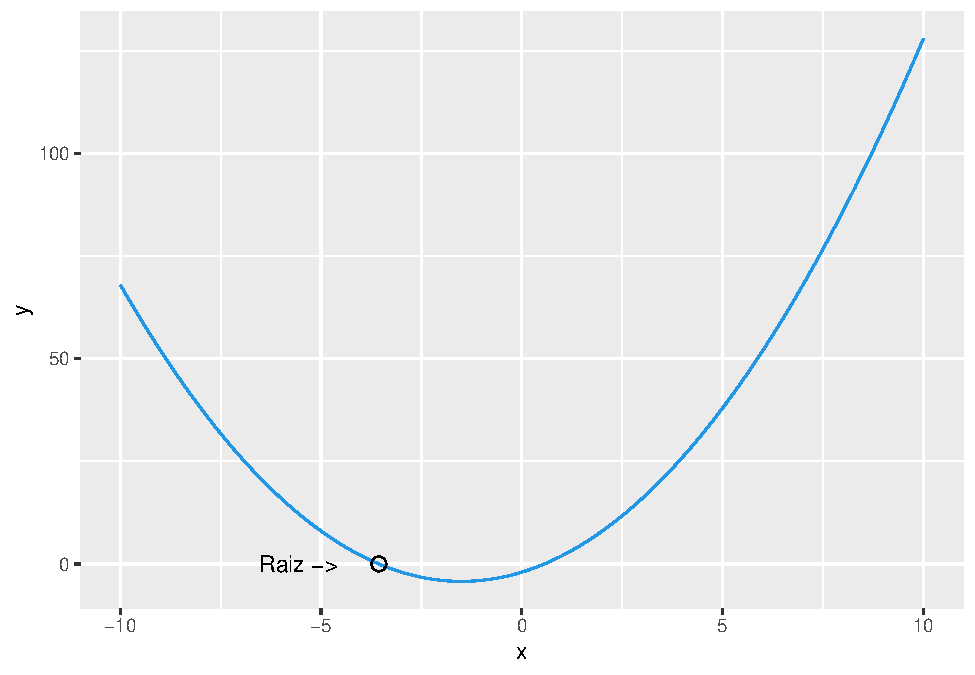
\includegraphics{Bisección_files/figure-latex/unnamed-chunk-4-1.pdf}

\newpage
\singlespacing 
\end{document}